%% VI STARTER MED ET HASH

\section{Turingmaskiner}%
\label{sec:turingmachines}

\subsection{Turingmaskiner}%
\label{subsec:label}



\begin{frame}
  \frametitle{Pensum}
  \begin{itemize}
    \item Sipser 3: \textbf{Turing Machines}
    \item Weekly Note 3
    \item Weekly Note 4
    \item Video 7-10
  \end{itemize}
\end{frame}

\begin{frame}[allowframebreaks]
  \frametitle{Turingmaskiner}
        \begin{itemize}
          \item En Turingmaskine er meget ligesom en PDA eller endelig automat, men med et tilknyttet uendeligt og ubegrænset bånd.
          \item Turingmaskinen genkender både regulære sprog samt kontekstfrie sprog, og alle afgørlige sprog (som vi kommer ind på senere).
          \item Turingmaskinens bånd:
                \begin{itemize}
                  \item Er uendeligt og ubegrænset
                  \item Har et hoved som kan flyttes til højre og venstre
                  \item Har en start, men ingen ende
                  \item Indeholder strengen og er blank alle andre steder
                  \item Kan skrives på (og slettes, ved at skrive \textit{det blanke tegn})
                \end{itemize}
          \item En anden vigtig forskel mellem endelige automater og Turingmaskiner, er at Turingmaskiners \textit{accept} og \textit{afvis} tilstande træder i kraft \textit{med det samme}.
        \end{itemize}
\end{frame}

\begin{frame}[allowframebreaks]
  \frametitle{Formel Definition af en Turingmaskine}
\begin{itemize}
  \item Hjertet af Turingmaskinen er dens overføringsfunktionen $\delta = Q \times \Gamma \longrightarrow Q \times \Gamma  \times \{L,R\}$
  \item Det vil sige, at hvis $\delta(q,a) = (r,b,L)$ går vi fra tilstand $q$ og hovedet er over $a$, skriver maskinen symbolet $b$ ved at erstatte $a$ og gå til tilstand $r$. $L$ og $R$ betyder at den enten går til venstre (L) eller højre (R)
\end{itemize}

\begin{definition}
  En Turingmaskine er en 7-tuple, $(Q, \Sigma, \Gamma, \delta, q_{0}, q_{accept}, q_{reject})$, hvor $Q, \Sigma, \Gamma$ alle er endelige mængder og
  \begin{enumerate}
    \item $Q$ er mængden af tilstande
    \item $\Sigma$ er inputalfabetet ikke indeholdende det \textit{blanke symbol} $\sqcup$
    \item $\Gamma$ er båndalfabetet hvor $\sqcup \in \Gamma$ og $\Sigma \subseteq \Gamma$.
    \item $\delta : Q \times \Gamma \longrightarrow Q \times \Gamma \times \{L,R\}$ er overføringsfunktionen
    \item $q_{0} \in Q$ er starttilstanden
    \item $q_{accept} \in Q$ er accepttilstanden, og
    \item $q_{reject} \in Q$ er afvisningstilstanden, hvor $q_{reject} \ne q_{accept}$.
  \end{enumerate}
\end{definition}

\begin{itemize}
  \item Komputeringen af en Turingmaskine $M$ fungerer som følger:
  \item Givet input $w = w_{1}w_{2} \ldots w_{n} \in \Sigma^{*}$ på båndets første $n$ felter.
  \item Resten af båndet er blankt.
  \item Hovedet starter på det venstremest felt af båndet.
  \item Da $\sqcup \notin \Sigma$ ved vi at input er færdigt når vi møder $\sqcup$
  \item Når $M$ starter kører den efter overføringsfunktionen.
  \item Hvis $M$ forsøger at bevæge sit hoved til venstre forbliver hovedet det samme sted.
        \begin{itemize}
          \item Nogle modeller siger at det ikke er tilladt, så instant \textit{afvis}.
        \end{itemize}
  \item Komputeringen bliver ved indtil den enten når en \textit{accept} eller \textit{afvis} tilstand, \textit{eller} den kører for evigt.
\end{itemize}
\end{frame}

\begin{frame}[allowframebreaks]
  \frametitle{Konfigurationer}

  \begin{itemize}
    \item En indstilling af en Turingmaskines tilstant, bånd og hovedlokation kaldes en \textit{konfiguration}.
    \item Konfigurationer skrives ofte på en special måde. Givet en tilstand $q$ og to strenge $u$ og $v$ over båndalfabetet $\Gamma$, skriver vi $uqv$ som konfigurationen hvor den nuværende tilstand er $q$, båndindeholdet er $uv$ og hovedets lokation er det første symbol i $v$.
    \item Lad os sige at vi har to konfigurationer, $C_{1}$ og $C_{2}$. Hvis vi kan gå fra $C_{1}$ til $C_{2}$ på ét skridt, siger vi at $C_{1}$ \textit{giver} $C_{2}$.
    \item \textbf{Eksempel}: Hvis $a, b, c \in \Gamma$ og $u, v \in \Gamma^{*}$ og $q_{i}, q_{j} \in Q$, så er $ua\,q_{i}\,bv$ og $u\,q_{j}\,acv$ to konfigurationer. Vi siger så at
          \begin{equation}
ua\,q_{i}\,bv \text{ giver } u\,q_{j}\,acv
          \end{equation}
          hvis overføringsfunktionen $\delta(q_{i},b) = (q_{j}, c, L)$. Omvendt kan vi sige at:
          \begin{equation}
ua\,q_{i}\,bv \text{ giver } uac\,q_{j}\,v
          \end{equation}
          hvis $\delta(q_{i}, b) = (q_{j}, c, R)$
    \item \textbf{Startkonfigurationen} af en Turingmaskine $M$ på input $w$ er konfigurationen $q_{0}w$. Dette indebærer altså at båndhovedets lokation er helt til venstre til at starte med.
    \item En \textbf{accepterende konfiguration} er en konfiguration hvor tilstanden er $q_{accept}$.
    \item En \textbf{afvisende konfiguration} er en konfiguration hvor tilstanden af kongiurationen er $q_{reject}$.
    \item Accepterende og afvisende konfigurationer er begge \textbf{standsende konfigurationer}, som betyder at de ikke giver andre konfigurationer.
  \end{itemize}
\end{frame}

\begin{frame}[allowframebreaks]
  \frametitle{Turingmaskiner, sprog}

  \begin{itemize}
    \item Samlingen af strenge som en Turingmaskine $M$ accepterer skrives $L(M)$ og kaldes \textit{sproget af $M$} eller \textit{sproget genkendt af $M$}.
  \end{itemize}

  \begin{definition}
Vi kalder et sprog \textit{Turing-genkendeligt} hvis en Turingmaskine genkender det.\footnote{Dette kaldes også rekursivt enumerabelt i noget litteratur.}
  \end{definition}

  \begin{itemize}
    \item Som tidligere sagt er der tre muligheder når en Turingmaskine kører. Enten \textit{accepterer} den, eller den \textit{afviser}, eller den \textit{løkker}, altså kører for evigt uden at standse.
    \item Nogle maskiner stopper på \textit{alle} inputs. Disse maskiner kalder vi \textit{afgørerer}, fordi de altid afgører en streng.
    \item En afgører som genkender et sprog siges at afgøre dette sprog.
  \end{itemize}

  \begin{definition}
Vi siger at et sprog er \textit{Turing-afgørligt} eller \textit{afgørligt} hvis en Turingmaskine afgører det.\footnote{Dette kaldes også et rekursivt sprog i noget litteratur.}
  \end{definition}

  \begin{itemize}
\item Det her kursus omhandler ikke Turingmaskinekonstruktion, så vi hopper over eksemplerne på Turingmaskiner.
  \end{itemize}
\end{frame}

\subsection{Varianter af Turingmaskiner}%
\label{subsec:label}

\begin{frame}
  \frametitle{Varianter af Turingmaskiner}
  \begin{itemize}
    \item Der findes flere varianter af Turingmaskiner:
          \begin{itemize}
            \item Flerbånds
            \item Dobbelt-sidetbånds
            \item Nondeterministiske
            \item Matrix
            \item Enumeratorer
          \end{itemize}


    \item Vi vil kigge på hver af disse uden meget detalje.
    \item En vigtig egenskab ved hver variant er at de \textit{alle er ækvivalente i deres beskrivelseskraft}.
  \end{itemize}
\end{frame}

\begin{frame}[allowframebreaks]
  \frametitle{Multibånd}

  \begin{itemize}
    \item En multibånds Turingmaskine er som en normal Turingmaskine, men med mere end ét bånd.
    \item Antallet af bånd må \textit{ikke} ændres under kørsel.
    \item Overføringsfunktionen ændres, så den kan køre på mere end ét bånd:
          \begin{equation}
\delta : Q \times \Gamma^{k} \longrightarrow Q \times \Gamma^{k} \times \{L, R, S\}^{k}
          \end{equation}
          hvor $k$ er antallet af bånd.
    \item Overføringsfunktionen fungerer ved at tage den nuværende tilstand i alle bånd og giver resultatet til alle bånd.
    \item For eksempel: $\delta(q_{i}, a_{1}, \ldots, a_{k}) = (q_{j}, b_{1}, \ldots, b_{k}, L, R, \ldots, L)$, hvor $b_{i}$ erstatter $a_{i}$ når hovedet bevæges. I Jørgens implementation tillader han også hovedet at stå stille (som man kan implementere ved at først udføre sin handling, gå en vej, og så udføre ingen handling, og gå tilbage).
    \item En multibånds Turingmaskine kan være hurtigere og mere intuitiv til nogle ting, såsom at kopiere en streng. Ved en sådan maskine kan dette gøres i $O(|w|)$ skridt, hvor det skal gøres på $O(|w|^{2})$ skridt i en normal deterministisk Turingmaskine.
  \end{itemize}

  \begin{theorem}
Hver multibånds Turingmaskine har en ækvivalent enkeltbånds Turingmaskine.
  \end{theorem}

  \begin{itemize}
\item Vi konstruerer en Turingmaskine $S$ der har samme funktionalitet som multibånds TM $M$.
    \item Lad antallet af bånd i $M$ være $k$:
    \item Lad $S$ bruge symbolet $\#$ til at indikere slut på et bånd, start på et nyt (i.e., $a\#b\#c$, hvor båndindholdet er $a,b,c$ for hhv. bånd $1,2,3$).
    \item $S$ skal holde styr på hovedets lokation på hvert bånd. Den gør dette ved et unikt symbol for hvert symbol. Her bruger vi en bolle over symbolet, e.g. $\overset{\circ}{b}$
    \item Så for eksempel vil $M$'s bånd have \texttt{\textbf{a}aaa}, \texttt{bbb\textbf{b}b} og $S$ vil så have $\overset{\circ}{a}aaa\#bbb\overset{\circ}{b}b\#$.
    \item Vi definerer nu hvordan $S$ komputere:
    \item $S = $ ``På input $w = w_{1} \ldots w_{n}$: \begin{enumerate}
                                                   \item Konvertér $S$ til et enkelt bånd
                                                   \item Simuler hver bevægelse:
                                                         \begin{enumerate}
                                                           \item Scan $S$ fra den første $\#$ til den $k+1$'e $\#$, som er i slutningen af båndet før det tomme symbol, så den kan finde ud af hvor hovederne er.
                                                           \item Lav en passthrough til at opdatere ifølge reglerne.
                                                           \item Hvis $S$ skal flytte til højre ud over en $\#$ laver den et rightshift.
                                                         \end{enumerate}
                                                 \end{enumerate}
\begin{itemize}
\end{itemize}
  \item Vi vil nu kigge i mere detalje på hvordan dette foregår.
  \item Følgende er en beskrivelse af en algoritme der kan konvertere enhver $k-$bånds Turingmaskine til en 1-bånds Turingmaskine:
        \begin{enumerate}
          \item Antag at $M$ er en $k$-bånds Turingmaskine
          \item For hver tilstand $q_{i}$ i $M$ har vi:
                \begin{enumerate}
                  \item Tilstande $q^{i}_{(\alpha_{1}, \alpha_{2}, \ldots \alpha_{k})}$ når $a_{i} \in \Gamma \cup \{-\}$, hvor $-$ betyder tomme eller endnu ikke kendt (altså vi ved ikke hvad der skal være der.)
                  \item Tilstande $p^{i}_{(\delta_{1}, \delta_{2}, \ldots, \delta_{k}, b_{1}, b_{2}, \ldots, b_{k}, \gamma_{1}, \gamma_{2}, \ldots, \gamma_{k})}$, hvor $\delta_{i} \in \Gamma \cup \{-\}$, $b_{i} \in \Gamma$, $\gamma_{i} \in \{R,L,S\}$. Så altså, det første \(\delta\) er enten båndsymboler eller ukendt, $b$ er båndsymboler og $\gamma$ er hovedbevægelser.
                \end{enumerate}
        \end{enumerate}
  \item For at forklare dybere:
    \item $(2.1)$: Når vi er i $q_{\beta_{1}, \beta_{2}, \ldots, \beta_{r}, -, -, \ldots, -}^{i}$ har vi indsamlet alle symbolerne under hovederne på de første $r$ bånd. Her betyder symbolerne $-$ igen at det er symboler vi endnu ikke kender.
    \item Altså betyder det at $\beta_{k}$ har hvad det simulerer bånd nummer $k$'s symbol under hovedet.
    \item $(2.2)$: Når vi er i $p^{i}_{(b_{1}, \ldots, b_{q}, -, \ldots, -, b_{1}, b_{2}, \ldots, b_{k}, \gamma_{1}, \gamma_{2}, \ldots, \gamma_{k})}$ har vi ændret båndcellerne under de første $q$ hoveder, og flyttet det $i$\emph{*} hoved $i \le q$ ifølge $\gamma_{i}$ og muligvis rightshifted.
    \item Altså, når vi er i den tilstand har vi allerede erstattet $a_{1}, \ldots, a_{q}$ med $b_{1}, \ldots, b_{q}$ og vi har flyttet hovederne ifølge reglerne $\delta_{1}, \delta_{k}$.
    \item Vi kan her se at der er mange mulige states. Til $q^{i}$ er der $(\Gamma+1)^{k}$ ($+1$ grundet $-$). Til $p^{i}$ er det $(\Gamma+1)^{k}+\Gamma^{k}+3^{k}$.
    \item Det er mange states, men det er polynomielt mange. Ikke eksponentielt.
    \item Lad os nu implementere ét skridt: $\delta(q_{i}, a_{1}, a_{2}, \ldots, a_{n}) = (q_{j}, b_{1}, b_{2}, \ldots, b_{k}, \gamma_{1}, \gamma_{2}, \ldots, \gamma_{k})$.

          \begin{enumerate}
            \item $M'$ starter i tilstanden $q^{i}_{(-,-, \ldots, -)}$ med konfigurationen $q^{i}w$ hvor $w$ er input
            \item I tilstanden $q^{i}(a_{1}, \ldots, a_{r}, -, \ldots, -)$ hvor $r < k$ flytter $M'$ dets hoved fremad til at kopiere indholdet under $M$'s $r+1$'e hoved. Dette er hukommelsen.
            \item Når vi når til state $q^{i}_{(a_{1}, a_{2}, \ldots, a_{k})}, a_{i} \in \Gamma$ har var samlet alle karakterer under $m$'s hoveder. Nu ændrer vi på disse symboler. Vi gør dette ved hjælp af en mellem-tilstands $p^{j}$. Vi går til tilstanden $p^{j}_{(-,\ldots,-,b_{1}, b_{2}, \ldots, b_{k}, \gamma_{1}, \gamma_{2}, \ldots, \gamma_{k})}$. Her ved vi endnu ikke hvad de første symboler der skal ændres er, men vi ved hvad de skal ændres til.
            \item I tilstanden $p^{j}_{b_{1}, \ldots, b_{s}, -, \ldots, -, b_{1}, b_{2}, \ldots, b_{k}, \gamma_{1}, \gamma_{2}, \ldots, \gamma_{k}}$ hvor $s < k$ gør vi følgende:
                  \begin{enumerate}
                    \item Flytter positionen af det $(s+1)$'e hoved.
                    \item Erstatter $a_{s+1}$ med $b_{s+1}$ og flytter hovedet $s+1$ i følge $\gamma_{s+1}$
                    \item Hvis $s+1 < k$ går vi til state $p^{j}_{(b_{1}, \ldots, b_{s+1}, \cdots, b_{1}, b_{2}, \ldots, b_{k}, \gamma_{1}, \ldots, \gamma_{k})}$ og tager skridt 4 om igen. Ellers flytter vi hovedet til den vestremest position og går til state $q^{j}_{(-, \ldots, -)}$
                  \end{enumerate}

          \end{enumerate}
    \item Køretiden for denne simulation er som følger:
          \begin{itemize}
            \item Vi tager $t$ skridt på input $w, |w| = n$.
            \item Båndet i denne turingmaskine kan have længde $n+t$ højest (da hvert skridt i værste tilfælde går til højre hver gang. )
            \item Vi kører frem og tilbage i båndet flere gange, for hvertr skridt kører vi frem én gang, så tilbage, så frem (for overføringsfunktionen) og så tilbage. Altså 4 gange.
            \item Dermed har ét skridt køretiden $O(\Sigma \text{ længden af båndet}) = O(n+kt)$ hvor $k$ er antal bånd
            \item Derudover er det muligt at vi skal lave rightshifts.
            \item Worst case shifter vi hver gang, hvilket giver os $(k-1)t + (k-2)t + \cdots + t = O(k^{2}t)$.
            \item Dermed er det samlede arbejde gjort på ét skridt $O(n+kt) + O(k^{2}t) = O(n+k^{2}t)$.
            \item Ved $t$ skridt vil det samlede arbejde for at simulere disse skridt være $O(nt + k^{2}t^{2})$, hvilket er \textit{polynomielt} i $n$ og $t$.
          \end{itemize}
  \end{itemize}

  \begin{corollary}
Et sprog er Turing-genkendeligt $\iff$ en multibånds Turingmaskine genkender det.
  \end{corollary}

  \begin{itemize}
    \item \(\Rightarrow\) Dette har vi lige bevist
    \item \(\Leftarrow\) En multibånds Turingmaskine fungerer også med ét bånd.
  \end{itemize}
\end{frame}

\begin{frame}[allowframebreaks]
  \frametitle{2-vejs Bånd}
  \begin{itemize}
    \item Er vi klar til et endnu længere bevis?
  \end{itemize}
\end{frame}

\begin{frame}
  \frametitle{2-vejs Bånd}
  \begin{itemize}
    \item Dog ikke: Det eneste vi skal vide her er at en 2-vejsbånds Turingmaskine også kan gå til venstre uendeligt langt, fordi båndet går uendeligt til begge sider.
  \end{itemize}
\end{frame}



\begin{frame}[allowframebreaks]
  \frametitle{Nondeterministisk}

  \begin{itemize}
    \item En Nondeterministisk Turingmaskine er ligesom en NFA og PDA, idet den kan \textit{gætte} sig frem til hvad den skal gøre som det næste.
    \item For hver tilstand er der $B = |Q| \cdot |\Gamma| \cdot 3$ mulige overføringer. Dermed kan overføringsfunktionen beskrives således:
          \begin{equation}
\delta : Q \times \Gamma \longrightarrow \mathcal{P}(Q \times \Gamma \times \{L,R,S\})
          \end{equation}
  \end{itemize}

  \begin{definition}
En nondeterministisk Turingmaskine (NDTM) $M$ genkender $L$ hvis $L = \{w \mid \exists \text{ en komputering for } M \text{ på } w \text{ der leder til } M \text{'s accepttilstand.}\}$
  \end{definition}

  \begin{itemize}
    \item Altså behøver et sprog ikke være afgørligt for at det er genkendeligt.
  \end{itemize}

  \begin{definition}
    En NDTM $M$ afgører $L$ hvis $\forall w \in \Sigma^{*}$:
    \begin{enumerate}
      \item $\exists k = k(M,w)$ således at $M$ aldrig tager mere end $k$ skridt på $w$, altså alle længder i træet har længde $\le k$.
      \item $w \in L \iff M$ har mindst én accepterende beregning på $w$.
    \end{enumerate}
  \end{definition}

  \begin{theorem}
Hver NDTM har en ækvivalent deterministisk TM.
  \end{theorem}

  \begin{itemize}
    \item :(
    \item Givet en deterministisk TM $D$ der er ækvivalent med en NDTM $N$, og $L(D) = L(N)$. Derudover: $D$ afgører $L \iff N$ afgører $L$.
    \item Vi vil gerne bevise ved at have en DTM $D$ til at simulere \textit{alle} grene i $N$.
    \item Vi bruger BFS til at simulere $N$ på $w$.
    \item Vi ved at dette er muligt, fordi hver tilstand har \textbf{højest} $B$ overføringer, eller ingen.
    \item Vi antager at hver overføring $\delta(q,a)$ har \textbf{præcis} $B$ overføringer, eller ingen.
    \item Givet antallet af overføringer $T \rightarrow \mathbb{N}$ på en tilstand $q$, hvis $T(q) < B$, kopierer vi den sidste state så $T(q) = B$.
    \item E.g. hvis $\delta(q,a) = \{(q,b,R)\}$ bliver dette til $\delta(q,a) = \{(q,b,R),(q,b,R),(q,b,R),(q,b,R)\}$
    \item For en given streng $g_{1}g_{2}\ldots g_{k}$ hvor $g_{i} \in \{1,2, \ldots, B\}$ kan vi simulere den korresponderende komputering af $N$ ved at tage det $g_{i}$'e valg på skridt $i$: Altså er en mulig streng $274$ hvilket betyder at vi i første skridt tager valg nummer 2, i det andet valg nummer 7, og i det tredje valg nummer 4. Vi vil fra denne streng også kunne deducere at $B \ge 7$ da 7 er det højeste tal i strengen.
    \item Vi kigger komputeringerne igennem ved at gå dem igennem lexicografisk (længde, så alfabetisk).
    \item I.e., først strenge af længde 1, så 2, så 3, og i disse længder, først 123, så 124, så 131, etc.
    \item Vi bliver ved med dette indtil vi finder en accepterende konfiguration.
    \item Vi kan holde styr på tallene ved at bruge båndet i Turingmaskinen.
    \item For eksempel kan strengen $223$ repræsenteres således:
          \begin{equation*}
\#00\#00\#000\#
          \end{equation*}
    \item Lad os nu konstruere $D$.
    \item $D$ vil have $3$ bånd:
          \begin{enumerate}
            \item Input
            \item $N$'s udregninger på $w$
            \item Tal base $B+1$
          \end{enumerate}
  \item Hvis $D$ er nået alle grene igennem og endnu ikke har fundet en accepterende konfiguration, så \textit{afvises} strengen.
  \item Lad os formalisere:
  \begin{enumerate}
    \item \begin{enumerate}
            \item $w_{1}w_{2} \ldots w_{n}$
            \item $\sqcup$
            \item $\#0\#$
          \end{enumerate}
    \item Kopiér bånd 1 til bånd 2
    \item Simulér $N$ på bånd 2 ved brug af tallene på bånd 3 til at vælge den næste overføring indtil én af følgende sker:
          \begin{itemize}
            \item Dead end
            \item $M$ accepteres
            \item $M$ afviser
            \item Der er ikke flere tal på bånd 3
          \end{itemize}
    \item Erstat $d_{1}, d_{2}, \ldots, d_{4}$ på bånd 3 med det næste i leksikografisk orden
    \item Gå til skridt 2
  \end{enumerate}
  \end{itemize}

  \begin{corollary}
Et sprog er Turing-genkendeligt $\iff$ en NDTM genkender det.
  \end{corollary}

  \begin{itemize}
    \item Enhver DTM er automatisk også en DTM
    \item Den anden retning har vi lige bevist.
    \item Hvor lang tid tager denne simulation af $N$ i $D$?
    \item Vi antager at $N$ kører i $r$ skridt.
    \item $D$ vil så højest simulere
          \begin{equation}
$B + B^{2} + \cdots + B^{r} \le B^{r+1}$
          \end{equation}

    \item Dette er eksponentiel tid
    \item $B$ kommer fra antallet af overføringer i første skridt, $B^{2}$ på andet skridt, etc.
  \end{itemize}


\end{frame}

\begin{frame}[allowframebreak]
  \frametitle{Et bånd med flere hoveder}
\begin{itemize}
  \item En anden variant tillader mere end ét hoved på ét bånd.
  \item Jeg har kun kigget på mine egne noter, men jeg har ikke bevist noget her. Jeg vil dog antage at måden vi kan simulere det ved en DTM er på samme måde som ved multibånds gør med flere hoveder.
\end{itemize}
\end{frame}

\begin{frame}[allowframebreaks]
  \frametitle{To-dimensionelt Bånd}
 \begin{itemize}
   \item Dennev ariant tillader en form for ``matrix'' lignende. Lidt lignende multibånds, men hvor der tillades uendelige bånd.
   \item Se evt. Figur 3.6 i mine noter, pp. 47
 \end{itemize}
\end{frame}

\begin{frame}[allowframebreaks]
  \frametitle{Universel Turingmaskine}
\begin{itemize}
  \item En universal Turingmaskine $U$ bruges til at simulere andre Turingmaskiner.
  \item $U$ har alfabetet $A^{*} = \{a_{1}, a_{2}, \cdots\}$ ud i det uendelige.
  \item $U$ har en universel mængde af tilstande: $Q^{*} = \{q_{1}, q_{2}, \cdots\}$ ud i det uendelige.
  \item Givet en TM $M = (Q, \Sigma, \Gamma, \delta, q_{0}, q_{acc}, q_{rej})$.
  \item Når $|Q| = r$ og $|\Gamma| = t$, kan vi redefinere $Q = \{q_{1}, q_{2}, \ldots, q_{r}\}$ og $\Gamma = \{a_{1}, a_{2}, \ldots, a_{t}\}$.
  \item Vi kan derfra konkludere at hver TM $M$ har en ækvivalent Turingmaskine $M'$ hvor $Q(M') \le Q^{*}$ og $\Gamma(M') \le \Gamma^{*}$
  \item Vi bruger binære tal til at repræsentere heltal, så $q_{7}$ ville være $q_{111}$.
  \item Når vi vil simulere en DTM koder vi overføringer som tupler. FOr eksempel: $\delta(q_{i}, a_{j}) = (q_{s}, a_{q}, \gamma)$ bliver til $((q_{i}, a_{j}), (q_{s}, a_{q}, \gamma))$, hvor $r = |Q(M)|, t = |\Gamma(M)|$.
  \item Vi antager at starttilstanden er $q_{1}$ og $q_{r-1}$ er accepttilstanden og $q_{r}$ er afvistilstanden.
  \item Vi kan med dette få en kodning af $M$ som vi kalder $\langle M \rangle$:
        \begin{equation*}
\langle M \rangle = (((q_{1}, a_{1}), (q_{f}, a_{q}, R)), ((q_{1}, a_{2}), \ldots), \ldots, (q_{r-2}, a_{t}), (q_{b}, a_{l}, L))
        \end{equation*}


  \item Vi kan også indkode strenge, e.g. $w \in \Gamma^{*}$: $w = a_{1}a_{2}a_{3}$, så er $\langle w \rangle = (a_{1}), (a_{2}), (a_{3})$
  \item Da vi bruger binære tal til kodning, betyder det at alle Turingmaskiner har følgende alfabet:
        \begin{equation*}
\Sigma = \{\text{\texttt{'(', ')', 'a', 'q', '0', '1', ',', 'R', 'L', 'S'}}\}
        \end{equation*}
  \item $U$ tager input af formen $\langle M,w \rangle$ og bruger 3 bånd til at simulere $M$ på $w$:
        \begin{enumerate}
          \item $\langle w\rangle $
          \item $\langle m \rangle $
          \item $q_{1}$
        \end{enumerate}

          \item Følgende er hvordan $U$ simulerer ét skridt af $M$:
                \begin{enumerate}
                  \item Lad $q$ være den tilstand der ligger på bånd 3
                  \item Lad $a$ være det symbol under hovedet på bånd 1
                  \item Find indtasting for $(q,a)$ på bånd 2, og udgær ændringer på båndene 1 og 3:
                        \begin{enumerate}
                          \item Hvis indtastningen er $((q,a), (p,b,L))$ så
                          \item Nyt symbol på bånd 1 er $b$ og hovedet bevæger sig til venstre.
                          \item Ny tilstand på bånd 3 er $p$
                        \end{enumerate}
                  \item Hvis $p = q_{r-1}$ går $U$ til accepttilstanden og stopper
                  \item Hvis $p = q_{r}$ så går $U$ ind i sin afvis tilstand og stopper.

                \end{enumerate}

\end{itemize}
\end{frame}

\begin{frame}[allowframebreaks]
  \frametitle{Enumeratorer}
\begin{itemize}
  \item En enumerator er en TM men med et tilknyttet output bånd. Altså kan den printe.
  \item En Enumerator vil altid køre for evigt, og printe forskellige strenge.
  \item Vi definerer sproget af en enumerator, $E$ til at være $L(E) = \{w \mid w \text{ er printet af } E\}$ i uendelig tid. $L$ er enumerabelt hvis $L = L(E)$ for en enumerator.
\end{itemize}

\begin{theorem}
$L$ er enumeralt $\iff$ $L$ er genkendeligt.
\end{theorem}

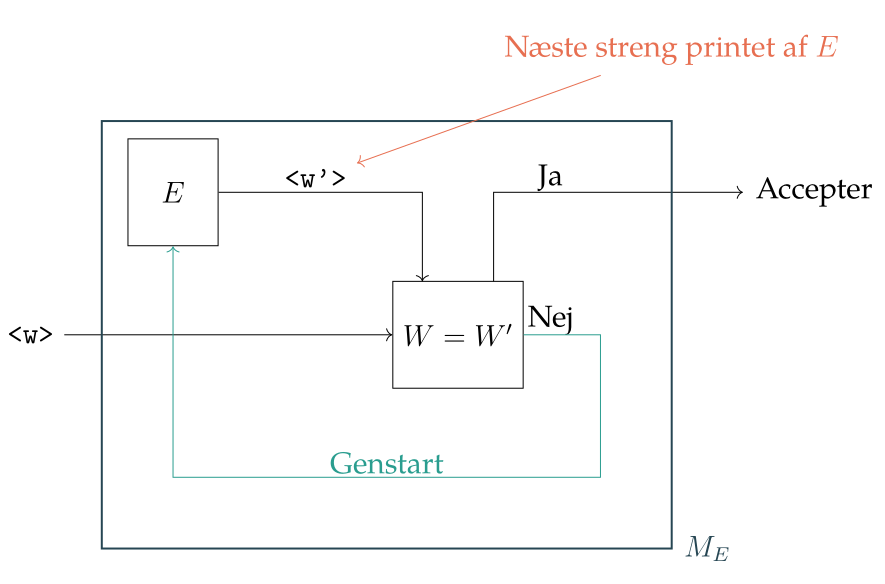
\includegraphics[scale=0.3]{figur/noter37.png}

\begin{itemize}
  \item Mere formelt, i.e., algoritmisk:
        \begin{enumerate}
          \item På input $\langle w \rangle$ starter TM $M_{E}$ enumerateren $E$ på den tomme streng.
          \item Når $E$ printer streng $w'$ sammenligner $M_{E}$ strengen $w'$ med $w$
          \item Hvis $w = w'$ så accepter $M_{e}$. Ellers genstarter den $E$ og venter på den næste streng $w'$ som bliver printet af $E$.
        \end{enumerate}

\end{itemize}
\end{frame}

\subsection{Definitionen af en Algoritme}%
\label{subsec:label}

\begin{frame}[allowframebreaks]
  \frametitle{Definitionen af en Algoritme}
  \begin{itemize}
    \item Resten af dette krusus vil ikke være om Turingmaskiner, men om algoritmer.
    \item Dog kan \textbf{alle} algoritmer der kan køre på en computer, køre på en Turingmaskine.
    \item Vi kan gøre dette ved at bruge en universel turing maskine, og en indkodning af de forskellige problemer.
    \item Et eksempel på en sådan kodning er sproget $A$ som er et sprog bestående af alle strenge der repræsenterer urettede grafer som er forbundne:
          \begin{equation*}
A = \{\langle G\rangle \mid G \text{ er en forbundet urettet graf}\}
          \end{equation*}

    \item Følgende er en højt-niveaus beskrivelse af en TM $M$ som afgører $A$:
    \item $M = $''På  input $\langle G \rangle$, kodning af en graf $G$:
          \begin{enumerate}
            \item Vælg den første knude af $G$ og markér den.
            \item Gentag den følgne fase indtil ingen nye knuder er markeret:
                  \begin{enumerate}
                    \item For hver knude i $G$ markér den hvis den er knyttet af en kant til en knude som allerede er markeret.
                  \end{enumerate}

            \item Scan alle knuderne af $G$ til at bestemme hvorvidt de alle er markeret. Hvis de er, så \textit{accepter}, ellers \textit{afvis}.
          \end{enumerate}

    \item Der er flere måder hvorpå vi kan kode en graf til at kunne køre denne algoritme, såsom at bruge en liste: \texttt{(1,2,3,4)((1,2),(2,3),(3,1),(1,4))} som koder følgende graf:

  \end{itemize}
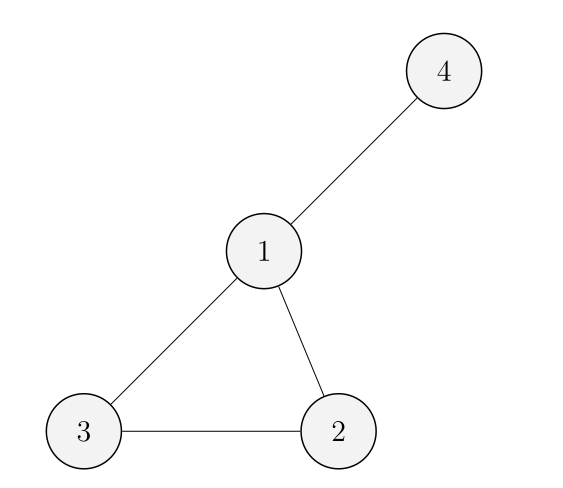
\includegraphics[scale=0.3]{figur/noter38.png}
\end{frame}

\begin{frame}[allowframebreaks]
  \frametitle{Hovedpointer}
\begin{itemize}
  \item En Turingmaskine (TM) er en automat hvis hoved kan bevæge sig til venstre
og højre. Derudover kan den ændre på sit bånd, som er uendeligt.
\item Turingmaskiner er langt mere kraftfulde end DFA’er og PDA’er. De er endda
accepteret som værende ligeså kraftfulde som moderne computere, hvilket
kommer fra Church-Turing tesen.
\item Turingmaskiner giver indsigt i de teoretiske grænser for komputering, altså
hvad en computer kan gøre, og hvor hurtigt den kan gøre det.
\item En Turingmaskine $M$ genkender et sprog $L \iff$ hver streng i $L$ leder $M$
til sin accepttilstand. Strenge ikke i $L$ leder enten til en afvis tilstand eller lader
$M$ køre i en løkke forevigt. $L(M )$ betegner sproget genkendt af $M$ . Bemærk
at alle Turingmaskiner genkender præcis ét sprog, nemlig det sæt af strenge
som den accepterer.
\item Et sprog $L$ kaldes genkendeligt hvis der er en Turingmaskine $M$ som
genkender $L$. Klassen af genkendelige sprog er sættet af alle sprog som er
genkendt af en Turingmaskine.
\item En Turingmaskine $M$ afgører et sprog $L \iff$ hver streng i $L$ leder $M$ til en
accept state og hver streng ikke i $L$ leder $M$ til en afvis tilstand. Altså betyder
det at $M$ stopper på alle strenge, og ikke kører uendeligt.
\item En afgører (decider) er en Turingmaskine som altid stopper (og dermed
ender i enten en accept eller afvis state.) Hver Turingmaskine som er en
afgører, afgører præcis ét sprog, nemlig sættet af strenge som ender i dens
accept state.
\item Et sprog $L$ kaldes afgørligt hvis der er en Turingmaskine $M$ som afgører
$L$. Klassen af afgørlige sprog er sættet af alle sprog som af afgjort af en
Turingmaskine.
\item Hvis et sprog er afgørligt, så er det også genkendeligt, men det omvendte
gælder ikke altid.
\item Der er forskellige måder at specificere en Turingmaskine på: Overføringstabel,
pseudokode, tilstandsdiagram og højtniveausbeskrivelser (som har været
hoveddelen af disse noter.)
\end{itemize}
\end{frame}



%%% Local Variables:
%%% mode: latex
%%% TeX-engine: xetex
%%% TeX-command-extra-options: "-shell-escape"
%%% TeX-master: "main"
%%% End:
